\documentclass[1p]{elsarticle_modified}
%\bibliographystyle{elsarticle-num}

%\usepackage[colorlinks]{hyperref}
%\usepackage{abbrmath_seonhwa} %\Abb, \Ascr, \Acal ,\Abf, \Afrak
\usepackage{amsfonts}
\usepackage{amssymb}
\usepackage{amsmath}
\usepackage{amsthm}
\usepackage{scalefnt}
\usepackage{amsbsy}
\usepackage{kotex}
\usepackage{caption}
\usepackage{subfig}
\usepackage{color}
\usepackage{graphicx}
\usepackage{xcolor} %% white, black, red, green, blue, cyan, magenta, yellow
\usepackage{float}
\usepackage{setspace}
\usepackage{hyperref}

\usepackage{tikz}
\usetikzlibrary{arrows}

\usepackage{multirow}
\usepackage{array} % fixed length table
\usepackage{hhline}

%%%%%%%%%%%%%%%%%%%%%
\makeatletter
\renewcommand*\env@matrix[1][\arraystretch]{%
	\edef\arraystretch{#1}%
	\hskip -\arraycolsep
	\let\@ifnextchar\new@ifnextchar
	\array{*\c@MaxMatrixCols c}}
\makeatother %https://tex.stackexchange.com/questions/14071/how-can-i-increase-the-line-spacing-in-a-matrix
%%%%%%%%%%%%%%%

\usepackage[normalem]{ulem}

\newcommand{\msout}[1]{\ifmmode\text{\sout{\ensuremath{#1}}}\else\sout{#1}\fi}
%SOURCE: \msout is \stkout macro in https://tex.stackexchange.com/questions/20609/strikeout-in-math-mode

\newcommand{\cancel}[1]{
	\ifmmode
	{\color{red}\msout{#1}}
	\else
	{\color{red}\sout{#1}}
	\fi
}

\newcommand{\add}[1]{
	{\color{blue}\uwave{#1}}
}

\newcommand{\replace}[2]{
	\ifmmode
	{\color{red}\msout{#1}}{\color{blue}\uwave{#2}}
	\else
	{\color{red}\sout{#1}}{\color{blue}\uwave{#2}}
	\fi
}

\newcommand{\Sol}{\mathcal{S}} %segment
\newcommand{\D}{D} %diagram
\newcommand{\A}{\mathcal{A}} %arc


%%%%%%%%%%%%%%%%%%%%%%%%%%%%%5 test

\def\sl{\operatorname{\textup{SL}}(2,\Cbb)}
\def\psl{\operatorname{\textup{PSL}}(2,\Cbb)}
\def\quan{\mkern 1mu \triangleright \mkern 1mu}

\theoremstyle{definition}
\newtheorem{thm}{Theorem}[section]
\newtheorem{prop}[thm]{Proposition}
\newtheorem{lem}[thm]{Lemma}
\newtheorem{ques}[thm]{Question}
\newtheorem{cor}[thm]{Corollary}
\newtheorem{defn}[thm]{Definition}
\newtheorem{exam}[thm]{Example}
\newtheorem{rmk}[thm]{Remark}
\newtheorem{alg}[thm]{Algorithm}

\newcommand{\I}{\sqrt{-1}}
\begin{document}

%\begin{frontmatter}
%
%\title{Boundary parabolic representations of knots up to 8 crossings}
%
%%% Group authors per affiliation:
%\author{Yunhi Cho} 
%\address{Department of Mathematics, University of Seoul, Seoul, Korea}
%\ead{yhcho@uos.ac.kr}
%
%
%\author{Seonhwa Kim} %\fnref{s_kim}}
%\address{Center for Geometry and Physics, Institute for Basic Science, Pohang, 37673, Korea}
%\ead{ryeona17@ibs.re.kr}
%
%\author{Hyuk Kim}
%\address{Department of Mathematical Sciences, Seoul National University, Seoul 08826, Korea}
%\ead{hyukkim@snu.ac.kr}
%
%\author{Seokbeom Yoon}
%\address{Department of Mathematical Sciences, Seoul National University, Seoul, 08826,  Korea}
%\ead{sbyoon15@snu.ac.kr}
%
%\begin{abstract}
%We find all boundary parabolic representation of knots up to 8 crossings.
%
%\end{abstract}
%\begin{keyword}
%    \MSC[2010] 57M25 
%\end{keyword}
%
%\end{frontmatter}

%\linenumbers
%\tableofcontents
%
\newcommand\colored[1]{\textcolor{white}{\rule[-0.35ex]{0.8em}{1.4ex}}\kern-0.8em\color{red} #1}%
%\newcommand\colored[1]{\textcolor{white}{ #1}\kern-2.17ex	\textcolor{white}{ #1}\kern-1.81ex	\textcolor{white}{ #1}\kern-2.15ex\color{red}#1	}

{\Large $\underline{12a_{0010}~(K12a_{0010})}$}

\setlength{\tabcolsep}{10pt}
\renewcommand{\arraystretch}{1.6}
\vspace{1cm}\begin{tabular}{m{100pt}>{\centering\arraybackslash}m{274pt}}
\multirow{5}{120pt}{
	\centering
	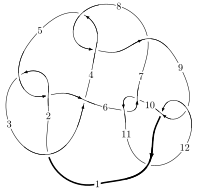
\includegraphics[width=112pt]{../../../GIT/diagram.site/Diagrams/png/811_12a_0010.png}\\
\ \ \ A knot diagram\footnotemark}&
\allowdisplaybreaks
\textbf{Linearized knot diagam} \\
\cline{2-2}
 &
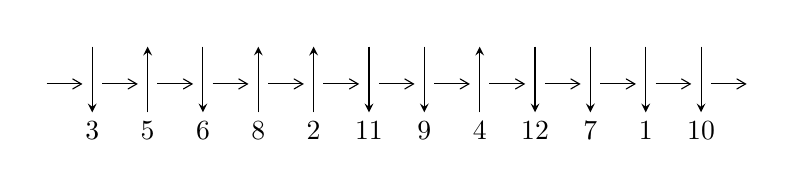
\begin{tikzpicture}[x=20pt, y=17pt]
	% nodes
	\node (C0) at (0, 0) {};
	\node (C1) at (1, 0) {};
	\node (C1U) at (1, +1) {};
	\node (C1D) at (1, -1) {3};

	\node (C2) at (2, 0) {};
	\node (C2U) at (2, +1) {};
	\node (C2D) at (2, -1) {5};

	\node (C3) at (3, 0) {};
	\node (C3U) at (3, +1) {};
	\node (C3D) at (3, -1) {6};

	\node (C4) at (4, 0) {};
	\node (C4U) at (4, +1) {};
	\node (C4D) at (4, -1) {8};

	\node (C5) at (5, 0) {};
	\node (C5U) at (5, +1) {};
	\node (C5D) at (5, -1) {2};

	\node (C6) at (6, 0) {};
	\node (C6U) at (6, +1) {};
	\node (C6D) at (6, -1) {11};

	\node (C7) at (7, 0) {};
	\node (C7U) at (7, +1) {};
	\node (C7D) at (7, -1) {9};

	\node (C8) at (8, 0) {};
	\node (C8U) at (8, +1) {};
	\node (C8D) at (8, -1) {4};

	\node (C9) at (9, 0) {};
	\node (C9U) at (9, +1) {};
	\node (C9D) at (9, -1) {12};

	\node (C10) at (10, 0) {};
	\node (C10U) at (10, +1) {};
	\node (C10D) at (10, -1) {7};

	\node (C11) at (11, 0) {};
	\node (C11U) at (11, +1) {};
	\node (C11D) at (11, -1) {1};

	\node (C12) at (12, 0) {};
	\node (C12U) at (12, +1) {};
	\node (C12D) at (12, -1) {10};
	\node (C13) at (13, 0) {};

	% arrows
	\draw[->,>={angle 60}]
	(C0) edge (C1) (C1) edge (C2) (C2) edge (C3) (C3) edge (C4) (C4) edge (C5) (C5) edge (C6) (C6) edge (C7) (C7) edge (C8) (C8) edge (C9) (C9) edge (C10) (C10) edge (C11) (C11) edge (C12) (C12) edge (C13) ;	\draw[->,>=stealth]
	(C1U) edge (C1D) (C2D) edge (C2U) (C3U) edge (C3D) (C4D) edge (C4U) (C5D) edge (C5U) (C6U) edge (C6D) (C7U) edge (C7D) (C8D) edge (C8U) (C9U) edge (C9D) (C10U) edge (C10D) (C11U) edge (C11D) (C12U) edge (C12D) ;
	\end{tikzpicture} \\
\hhline{~~} \\& 
\textbf{Solving Sequence} \\ \cline{2-2} 
 &
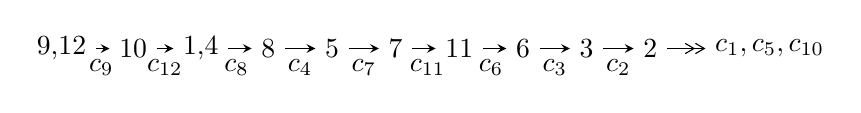
\begin{tikzpicture}[x=23pt, y=7pt]
	% node
	\node (A0) at (-1/8, 0) {9,12};
	\node (A1) at (1, 0) {10};
	\node (A2) at (33/16, 0) {1,4};
	\node (A3) at (25/8, 0) {8};
	\node (A4) at (33/8, 0) {5};
	\node (A5) at (41/8, 0) {7};
	\node (A6) at (49/8, 0) {11};
	\node (A7) at (57/8, 0) {6};
	\node (A8) at (65/8, 0) {3};
	\node (A9) at (73/8, 0) {2};
	\node (C1) at (1/2, -1) {$c_{9}$};
	\node (C2) at (3/2, -1) {$c_{12}$};
	\node (C3) at (21/8, -1) {$c_{8}$};
	\node (C4) at (29/8, -1) {$c_{4}$};
	\node (C5) at (37/8, -1) {$c_{7}$};
	\node (C6) at (45/8, -1) {$c_{11}$};
	\node (C7) at (53/8, -1) {$c_{6}$};
	\node (C8) at (61/8, -1) {$c_{3}$};
	\node (C9) at (69/8, -1) {$c_{2}$};
	\node (A10) at (11, 0) {$c_{1},c_{5},c_{10}$};

	% edge
	\draw[->,>=stealth]	
	(A0) edge (A1) (A1) edge (A2) (A2) edge (A3) (A3) edge (A4) (A4) edge (A5) (A5) edge (A6) (A6) edge (A7) (A7) edge (A8) (A8) edge (A9) ;
	\draw[->>,>={angle 60}]	
	(A9) edge (A10);
\end{tikzpicture} \\ 

\end{tabular} \\

\footnotetext{
The image of knot diagram is generated by the software ``\textbf{Draw programme}" developed by Andrew Bartholomew(\url{http://www.layer8.co.uk/maths/draw/index.htm\#Running-draw}), where we modified some parts for our purpose(\url{https://github.com/CATsTAILs/LinksPainter}).
}\phantom \\ \newline 
\centering \textbf{Ideals for irreducible components\footnotemark of $X_{\text{par}}$} 
 
\begin{align*}
I^u_{1}&=\langle 
1.53494\times10^{76} u^{118}+2.11404\times10^{77} u^{117}+\cdots+6.29838\times10^{74} b-4.20588\times10^{76},\\
\phantom{I^u_{1}}&\phantom{= \langle  }-3.27734\times10^{76} u^{118}-1.76333\times10^{77} u^{117}+\cdots+3.14919\times10^{74} a-2.34713\times10^{77},\\
\phantom{I^u_{1}}&\phantom{= \langle  }u^{119}+13 u^{118}+\cdots-20 u-1\rangle \\
I^u_{2}&=\langle 
- a^3- a^2+b- a,\;a^4+a^3+a^2+1,\;u-1\rangle \\
I^u_{3}&=\langle 
b,\;u^2 a+a^2+2 a u+3 u^2+a+5 u+4,\;u^3+u^2-1\rangle \\
I^u_{4}&=\langle 
- a^5+2 a^4-2 a^3+2 a^2+b-2 a+1,\;a^6-2 a^5+2 a^4-2 a^3+2 a^2- a+1,\;u-1\rangle \\
\\
\end{align*}
\raggedright * 4 irreducible components of $\dim_{\mathbb{C}}=0$, with total 135 representations.\\
\footnotetext{All coefficients of polynomials are rational numbers. But the coefficients are sometimes approximated in decimal forms when there is not enough margin.}
\newpage
\renewcommand{\arraystretch}{1}
\centering \section*{I. $I^u_{1}= \langle 1.53\times10^{76} u^{118}+2.11\times10^{77} u^{117}+\cdots+6.30\times10^{74} b-4.21\times10^{76},\;-3.28\times10^{76} u^{118}-1.76\times10^{77} u^{117}+\cdots+3.15\times10^{74} a-2.35\times10^{77},\;u^{119}+13 u^{118}+\cdots-20 u-1 \rangle$}
\flushleft \textbf{(i) Arc colorings}\\
\begin{tabular}{m{7pt} m{180pt} m{7pt} m{180pt} }
\flushright $a_{9}=$&$\begin{pmatrix}1\\0\end{pmatrix}$ \\
\flushright $a_{12}=$&$\begin{pmatrix}0\\u\end{pmatrix}$ \\
\flushright $a_{10}=$&$\begin{pmatrix}1\\u^2\end{pmatrix}$ \\
\flushright $a_{1}=$&$\begin{pmatrix}- u\\- u^3+u\end{pmatrix}$ \\
\flushright $a_{4}=$&$\begin{pmatrix}104.069 u^{118}+559.930 u^{117}+\cdots+12845.3 u+745.312\\-24.3704 u^{118}-335.648 u^{117}+\cdots+1158.29 u+66.7771\end{pmatrix}$ \\
\flushright $a_{8}=$&$\begin{pmatrix}148.115 u^{118}+1786.08 u^{117}+\cdots-3799.29 u-227.176\\27.5034 u^{118}+486.129 u^{117}+\cdots-4211.15 u-238.606\end{pmatrix}$ \\
\flushright $a_{5}=$&$\begin{pmatrix}509.194 u^{118}+5592.67 u^{117}+\cdots+4807.30 u+342.681\\332.399 u^{118}+4415.95 u^{117}+\cdots-11668.3 u-608.640\end{pmatrix}$ \\
\flushright $a_{7}=$&$\begin{pmatrix}175.618 u^{118}+2272.21 u^{117}+\cdots-8010.44 u-465.782\\27.5034 u^{118}+486.129 u^{117}+\cdots-4211.15 u-238.606\end{pmatrix}$ \\
\flushright $a_{11}=$&$\begin{pmatrix}u^3\\u^5- u^3+u\end{pmatrix}$ \\
\flushright $a_{6}=$&$\begin{pmatrix}99.1977 u^{118}+1386.25 u^{117}+\cdots-7021.64 u-412.862\\-67.9945 u^{118}-781.463 u^{117}+\cdots-702.392 u-51.4383\end{pmatrix}$ \\
\flushright $a_{3}=$&$\begin{pmatrix}928.371 u^{118}+10559.2 u^{117}+\cdots-672.763 u+54.6534\\660.964 u^{118}+8651.81 u^{117}+\cdots-22541.4 u-1190.83\end{pmatrix}$ \\
\flushright $a_{2}=$&$\begin{pmatrix}466.460 u^{118}+5235.90 u^{117}+\cdots+1169.98 u+102.276\\557.127 u^{118}+7140.14 u^{117}+\cdots-16297.2 u-860.184\end{pmatrix}$\\&\end{tabular}
\flushleft \textbf{(ii) Obstruction class $= -1$}\\~\\
\flushleft \textbf{(iii) Cusp Shapes $= 413.566 u^{118}+3160.04 u^{117}+\cdots+29822.9 u+1714.64$}\\~\\
\newpage\renewcommand{\arraystretch}{1}
\flushleft \textbf{(iv) u-Polynomials at the component}\newline \\
\begin{tabular}{m{50pt}|m{274pt}}
Crossings & \hspace{64pt}u-Polynomials at each crossing \\
\hline $$\begin{aligned}c_{1}\end{aligned}$$&$\begin{aligned}
&u^{119}+55 u^{118}+\cdots+208 u-1
\end{aligned}$\\
\hline $$\begin{aligned}c_{2},c_{5}\end{aligned}$$&$\begin{aligned}
&u^{119}+5 u^{118}+\cdots+8 u-1
\end{aligned}$\\
\hline $$\begin{aligned}c_{3}\end{aligned}$$&$\begin{aligned}
&u^{119}-5 u^{118}+\cdots+5788 u-292
\end{aligned}$\\
\hline $$\begin{aligned}c_{4},c_{8}\end{aligned}$$&$\begin{aligned}
&u^{119}-2 u^{118}+\cdots+32 u+64
\end{aligned}$\\
\hline $$\begin{aligned}c_{6},c_{10}\end{aligned}$$&$\begin{aligned}
&u^{119}-3 u^{118}+\cdots-5120 u+1024
\end{aligned}$\\
\hline $$\begin{aligned}c_{7}\end{aligned}$$&$\begin{aligned}
&u^{119}+40 u^{118}+\cdots-80896 u-4096
\end{aligned}$\\
\hline $$\begin{aligned}c_{9},c_{12}\end{aligned}$$&$\begin{aligned}
&u^{119}-13 u^{118}+\cdots-20 u+1
\end{aligned}$\\
\hline $$\begin{aligned}c_{11}\end{aligned}$$&$\begin{aligned}
&u^{119}+53 u^{118}+\cdots-14 u+1
\end{aligned}$\\
\hline
\end{tabular}\\~\\
\newpage\renewcommand{\arraystretch}{1}
\flushleft \textbf{(v) Riley Polynomials at the component}\newline \\
\begin{tabular}{m{50pt}|m{274pt}}
Crossings & \hspace{64pt}Riley Polynomials at each crossing \\
\hline $$\begin{aligned}c_{1}\end{aligned}$$&$\begin{aligned}
&y^{119}+23 y^{118}+\cdots+45340 y-1
\end{aligned}$\\
\hline $$\begin{aligned}c_{2},c_{5}\end{aligned}$$&$\begin{aligned}
&y^{119}+55 y^{118}+\cdots+208 y-1
\end{aligned}$\\
\hline $$\begin{aligned}c_{3}\end{aligned}$$&$\begin{aligned}
&y^{119}-9 y^{118}+\cdots+26282120 y-85264
\end{aligned}$\\
\hline $$\begin{aligned}c_{4},c_{8}\end{aligned}$$&$\begin{aligned}
&y^{119}+40 y^{118}+\cdots-80896 y-4096
\end{aligned}$\\
\hline $$\begin{aligned}c_{6},c_{10}\end{aligned}$$&$\begin{aligned}
&y^{119}+69 y^{118}+\cdots-31981568 y-1048576
\end{aligned}$\\
\hline $$\begin{aligned}c_{7}\end{aligned}$$&$\begin{aligned}
&y^{119}+68 y^{118}+\cdots+5134876672 y-16777216
\end{aligned}$\\
\hline $$\begin{aligned}c_{9},c_{12}\end{aligned}$$&$\begin{aligned}
&y^{119}-53 y^{118}+\cdots-14 y-1
\end{aligned}$\\
\hline $$\begin{aligned}c_{11}\end{aligned}$$&$\begin{aligned}
&y^{119}+39 y^{118}+\cdots+5618 y-1
\end{aligned}$\\
\hline
\end{tabular}\\~\\
\newpage\flushleft \textbf{(vi) Complex Volumes and Cusp Shapes}
$$\begin{array}{c|c|c}  
\text{Solutions to }I^u_{1}& \I (\text{vol} + \sqrt{-1}CS) & \text{Cusp shape}\\
 \hline 
\begin{aligned}
u &= \phantom{-}0.839718 + 0.548941 I \\
a &= \phantom{-}1.03007 + 1.37383 I \\
b &= -0.794811 - 0.704672 I\end{aligned}
 & \phantom{-}1.89954 - 0.71334 I & \phantom{-0.000000 } 0 \\ \hline\begin{aligned}
u &= \phantom{-}0.839718 - 0.548941 I \\
a &= \phantom{-}1.03007 - 1.37383 I \\
b &= -0.794811 + 0.704672 I\end{aligned}
 & \phantom{-}1.89954 + 0.71334 I & \phantom{-0.000000 } 0 \\ \hline\begin{aligned}
u &= -0.414192 + 0.897221 I \\
a &= \phantom{-}1.060200 - 0.496479 I \\
b &= -0.687708 + 1.025140 I\end{aligned}
 & \phantom{-}0.91210 - 4.63467 I & \phantom{-0.000000 } 0 \\ \hline\begin{aligned}
u &= -0.414192 - 0.897221 I \\
a &= \phantom{-}1.060200 + 0.496479 I \\
b &= -0.687708 - 1.025140 I\end{aligned}
 & \phantom{-}0.91210 + 4.63467 I & \phantom{-0.000000 } 0 \\ \hline\begin{aligned}
u &= -0.835785 + 0.571845 I \\
a &= \phantom{-}0.665117 - 0.447173 I \\
b &= -0.834943 - 0.140628 I\end{aligned}
 & \phantom{-}1.84382 + 2.29296 I & \phantom{-0.000000 } 0 \\ \hline\begin{aligned}
u &= -0.835785 - 0.571845 I \\
a &= \phantom{-}0.665117 + 0.447173 I \\
b &= -0.834943 + 0.140628 I\end{aligned}
 & \phantom{-}1.84382 - 2.29296 I & \phantom{-0.000000 } 0 \\ \hline\begin{aligned}
u &= -0.479737 + 0.894115 I \\
a &= \phantom{-}1.68069 + 0.21651 I \\
b &= -0.948305 - 0.723106 I\end{aligned}
 & \phantom{-}5.19353 - 5.82530 I & \phantom{-0.000000 } 0 \\ \hline\begin{aligned}
u &= -0.479737 - 0.894115 I \\
a &= \phantom{-}1.68069 - 0.21651 I \\
b &= -0.948305 + 0.723106 I\end{aligned}
 & \phantom{-}5.19353 + 5.82530 I & \phantom{-0.000000 } 0 \\ \hline\begin{aligned}
u &= \phantom{-}0.859164 + 0.551104 I \\
a &= \phantom{-}2.56167 + 0.36793 I \\
b &= -0.692210 + 0.826381 I\end{aligned}
 & \phantom{-}1.83580 - 3.70893 I & \phantom{-0.000000 } 0 \\ \hline\begin{aligned}
u &= \phantom{-}0.859164 - 0.551104 I \\
a &= \phantom{-}2.56167 - 0.36793 I \\
b &= -0.692210 - 0.826381 I\end{aligned}
 & \phantom{-}1.83580 + 3.70893 I & \phantom{-0.000000 } 0\\
 \hline 
 \end{array}$$\newpage$$\begin{array}{c|c|c}  
\text{Solutions to }I^u_{1}& \I (\text{vol} + \sqrt{-1}CS) & \text{Cusp shape}\\
 \hline 
\begin{aligned}
u &= \phantom{-}0.920082 + 0.330594 I \\
a &= -1.05886 - 1.09117 I \\
b &= \phantom{-}0.701252 + 0.313348 I\end{aligned}
 & -2.14764 + 0.46525 I & \phantom{-0.000000 } 0 \\ \hline\begin{aligned}
u &= \phantom{-}0.920082 - 0.330594 I \\
a &= -1.05886 + 1.09117 I \\
b &= \phantom{-}0.701252 - 0.313348 I\end{aligned}
 & -2.14764 - 0.46525 I & \phantom{-0.000000 } 0 \\ \hline\begin{aligned}
u &= -0.535990 + 0.870642 I \\
a &= \phantom{-}1.351430 - 0.147219 I \\
b &= -0.718212 + 0.865805 I\end{aligned}
 & \phantom{-}5.58089 + 1.54128 I & \phantom{-0.000000 } 0 \\ \hline\begin{aligned}
u &= -0.535990 - 0.870642 I \\
a &= \phantom{-}1.351430 + 0.147219 I \\
b &= -0.718212 - 0.865805 I\end{aligned}
 & \phantom{-}5.58089 - 1.54128 I & \phantom{-0.000000 } 0 \\ \hline\begin{aligned}
u &= -0.811525 + 0.533856 I \\
a &= -0.006008 + 1.406260 I \\
b &= -0.202031 + 0.895750 I\end{aligned}
 & \phantom{-}1.40789 - 0.40488 I & \phantom{-0.000000 } 0 \\ \hline\begin{aligned}
u &= -0.811525 - 0.533856 I \\
a &= -0.006008 - 1.406260 I \\
b &= -0.202031 - 0.895750 I\end{aligned}
 & \phantom{-}1.40789 + 0.40488 I & \phantom{-0.000000 } 0 \\ \hline\begin{aligned}
u &= -0.506849 + 0.899088 I \\
a &= -1.324780 + 0.302703 I \\
b &= \phantom{-}0.743370 - 0.916592 I\end{aligned}
 & \phantom{-}6.96695 - 3.78303 I & \phantom{-0.000000 } 0 \\ \hline\begin{aligned}
u &= -0.506849 - 0.899088 I \\
a &= -1.324780 - 0.302703 I \\
b &= \phantom{-}0.743370 + 0.916592 I\end{aligned}
 & \phantom{-}6.96695 + 3.78303 I & \phantom{-0.000000 } 0 \\ \hline\begin{aligned}
u &= -0.520633 + 0.894920 I \\
a &= -1.58006 - 0.26157 I \\
b &= \phantom{-}0.896350 + 0.744474 I\end{aligned}
 & \phantom{-}7.05859 - 0.70677 I & \phantom{-0.000000 } 0 \\ \hline\begin{aligned}
u &= -0.520633 - 0.894920 I \\
a &= -1.58006 + 0.26157 I \\
b &= \phantom{-}0.896350 - 0.744474 I\end{aligned}
 & \phantom{-}7.05859 + 0.70677 I & \phantom{-0.000000 } 0\\
 \hline 
 \end{array}$$\newpage$$\begin{array}{c|c|c}  
\text{Solutions to }I^u_{1}& \I (\text{vol} + \sqrt{-1}CS) & \text{Cusp shape}\\
 \hline 
\begin{aligned}
u &= \phantom{-}0.700245 + 0.663386 I \\
a &= -0.88509 - 1.53838 I \\
b &= \phantom{-}0.659039 + 0.972129 I\end{aligned}
 & -0.29156 + 6.55308 I & \phantom{-0.000000 } 0 \\ \hline\begin{aligned}
u &= \phantom{-}0.700245 - 0.663386 I \\
a &= -0.88509 + 1.53838 I \\
b &= \phantom{-}0.659039 - 0.972129 I\end{aligned}
 & -0.29156 - 6.55308 I & \phantom{-0.000000 } 0 \\ \hline\begin{aligned}
u &= -0.880230 + 0.554713 I \\
a &= \phantom{-}0.36352 - 1.59110 I \\
b &= \phantom{-}0.057310 - 0.897606 I\end{aligned}
 & \phantom{-}1.17161 + 4.80695 I & \phantom{-0.000000 } 0 \\ \hline\begin{aligned}
u &= -0.880230 - 0.554713 I \\
a &= \phantom{-}0.36352 + 1.59110 I \\
b &= \phantom{-}0.057310 + 0.897606 I\end{aligned}
 & \phantom{-}1.17161 - 4.80695 I & \phantom{-0.000000 } 0 \\ \hline\begin{aligned}
u &= -0.563327 + 0.775350 I \\
a &= \phantom{-}1.353100 - 0.003460 I \\
b &= -0.815150 - 0.602192 I\end{aligned}
 & \phantom{-}2.15561 + 0.96157 I & \phantom{-0.000000 } 0 \\ \hline\begin{aligned}
u &= -0.563327 - 0.775350 I \\
a &= \phantom{-}1.353100 + 0.003460 I \\
b &= -0.815150 + 0.602192 I\end{aligned}
 & \phantom{-}2.15561 - 0.96157 I & \phantom{-0.000000 } 0 \\ \hline\begin{aligned}
u &= \phantom{-}0.729173 + 0.618822 I \\
a &= \phantom{-}0.91485 + 1.48291 I \\
b &= -0.677218 - 0.888176 I\end{aligned}
 & \phantom{-}1.64414 + 1.56779 I & \phantom{-0.000000 } 0 \\ \hline\begin{aligned}
u &= \phantom{-}0.729173 - 0.618822 I \\
a &= \phantom{-}0.91485 - 1.48291 I \\
b &= -0.677218 + 0.888176 I\end{aligned}
 & \phantom{-}1.64414 - 1.56779 I & \phantom{-0.000000 } 0 \\ \hline\begin{aligned}
u &= \phantom{-}0.806433 + 0.513028 I \\
a &= -2.73489 - 0.49333 I \\
b &= \phantom{-}0.677943 - 0.716615 I\end{aligned}
 & \phantom{-}0.49484 + 1.35815 I & \phantom{-0.000000 } 0 \\ \hline\begin{aligned}
u &= \phantom{-}0.806433 - 0.513028 I \\
a &= -2.73489 + 0.49333 I \\
b &= \phantom{-}0.677943 + 0.716615 I\end{aligned}
 & \phantom{-}0.49484 - 1.35815 I & \phantom{-0.000000 } 0\\
 \hline 
 \end{array}$$\newpage$$\begin{array}{c|c|c}  
\text{Solutions to }I^u_{1}& \I (\text{vol} + \sqrt{-1}CS) & \text{Cusp shape}\\
 \hline 
\begin{aligned}
u &= \phantom{-}0.896751 + 0.539049 I \\
a &= -1.09612 - 1.34285 I \\
b &= \phantom{-}0.874636 + 0.641589 I\end{aligned}
 & \phantom{-}0.17888 - 5.63399 I & \phantom{-0.000000 } 0 \\ \hline\begin{aligned}
u &= \phantom{-}0.896751 - 0.539049 I \\
a &= -1.09612 + 1.34285 I \\
b &= \phantom{-}0.874636 - 0.641589 I\end{aligned}
 & \phantom{-}0.17888 + 5.63399 I & \phantom{-0.000000 } 0 \\ \hline\begin{aligned}
u &= -0.449457 + 0.951285 I \\
a &= -1.264510 + 0.571043 I \\
b &= \phantom{-}0.774340 - 1.021660 I\end{aligned}
 & \phantom{-}6.17714 - 6.89104 I & \phantom{-0.000000 } 0 \\ \hline\begin{aligned}
u &= -0.449457 - 0.951285 I \\
a &= -1.264510 - 0.571043 I \\
b &= \phantom{-}0.774340 + 1.021660 I\end{aligned}
 & \phantom{-}6.17714 + 6.89104 I & \phantom{-0.000000 } 0 \\ \hline\begin{aligned}
u &= -0.432123 + 0.970962 I \\
a &= \phantom{-}1.25415 - 0.65761 I \\
b &= -0.785309 + 1.057920 I\end{aligned}
 & \phantom{-}4.11704 - 12.19560 I & \phantom{-0.000000 } 0 \\ \hline\begin{aligned}
u &= -0.432123 - 0.970962 I \\
a &= \phantom{-}1.25415 + 0.65761 I \\
b &= -0.785309 - 1.057920 I\end{aligned}
 & \phantom{-}4.11704 + 12.19560 I & \phantom{-0.000000 } 0 \\ \hline\begin{aligned}
u &= -0.935084 + 0.512602 I \\
a &= -0.632458 + 0.577496 I \\
b &= \phantom{-}1.039780 - 0.012368 I\end{aligned}
 & -1.16555 + 5.57300 I & \phantom{-0.000000 } 0 \\ \hline\begin{aligned}
u &= -0.935084 - 0.512602 I \\
a &= -0.632458 - 0.577496 I \\
b &= \phantom{-}1.039780 + 0.012368 I\end{aligned}
 & -1.16555 - 5.57300 I & \phantom{-0.000000 } 0 \\ \hline\begin{aligned}
u &= -0.810344 + 0.451943 I \\
a &= -0.728244 + 0.571667 I \\
b &= \phantom{-}1.018150 + 0.257504 I\end{aligned}
 & -0.64746 - 1.61824 I & \phantom{-0.000000 } 0 \\ \hline\begin{aligned}
u &= -0.810344 - 0.451943 I \\
a &= -0.728244 - 0.571667 I \\
b &= \phantom{-}1.018150 - 0.257504 I\end{aligned}
 & -0.64746 + 1.61824 I & \phantom{-0.000000 } 0\\
 \hline 
 \end{array}$$\newpage$$\begin{array}{c|c|c}  
\text{Solutions to }I^u_{1}& \I (\text{vol} + \sqrt{-1}CS) & \text{Cusp shape}\\
 \hline 
\begin{aligned}
u &= -0.857581 + 0.325966 I \\
a &= \phantom{-}0.188149 - 0.845340 I \\
b &= \phantom{-}0.348024 - 1.228190 I\end{aligned}
 & -5.56356 + 0.94413 I & \phantom{-0.000000 } 0 \\ \hline\begin{aligned}
u &= -0.857581 - 0.325966 I \\
a &= \phantom{-}0.188149 + 0.845340 I \\
b &= \phantom{-}0.348024 + 1.228190 I\end{aligned}
 & -5.56356 - 0.94413 I & \phantom{-0.000000 } 0 \\ \hline\begin{aligned}
u &= \phantom{-}1.073860 + 0.172674 I \\
a &= \phantom{-}1.16829 + 1.04677 I \\
b &= -0.698025 + 0.105091 I\end{aligned}
 & -2.63266 - 2.23010 I & \phantom{-0.000000 } 0 \\ \hline\begin{aligned}
u &= \phantom{-}1.073860 - 0.172674 I \\
a &= \phantom{-}1.16829 - 1.04677 I \\
b &= -0.698025 - 0.105091 I\end{aligned}
 & -2.63266 + 2.23010 I & \phantom{-0.000000 } 0 \\ \hline\begin{aligned}
u &= -0.612148 + 0.916355 I \\
a &= -1.36804 - 0.41960 I \\
b &= \phantom{-}0.767030 + 0.815475 I\end{aligned}
 & \phantom{-}7.27557 + 1.92163 I & \phantom{-0.000000 } 0 \\ \hline\begin{aligned}
u &= -0.612148 - 0.916355 I \\
a &= -1.36804 + 0.41960 I \\
b &= \phantom{-}0.767030 - 0.815475 I\end{aligned}
 & \phantom{-}7.27557 - 1.92163 I & \phantom{-0.000000 } 0 \\ \hline\begin{aligned}
u &= \phantom{-}0.895015 + 0.056762 I \\
a &= -0.97632 - 4.21446 I \\
b &= \phantom{-}0.037868 - 0.362547 I\end{aligned}
 & -1.30782 - 2.14757 I & \phantom{-0.000000 } 0 \\ \hline\begin{aligned}
u &= \phantom{-}0.895015 - 0.056762 I \\
a &= -0.97632 + 4.21446 I \\
b &= \phantom{-}0.037868 + 0.362547 I\end{aligned}
 & -1.30782 + 2.14757 I & \phantom{-0.000000 } 0 \\ \hline\begin{aligned}
u &= \phantom{-}0.938429 + 0.604225 I \\
a &= \phantom{-}2.35579 + 0.15592 I \\
b &= -0.711352 + 0.998662 I\end{aligned}
 & \phantom{-}0.99788 - 6.39299 I & \phantom{-0.000000 } 0 \\ \hline\begin{aligned}
u &= \phantom{-}0.938429 - 0.604225 I \\
a &= \phantom{-}2.35579 - 0.15592 I \\
b &= -0.711352 - 0.998662 I\end{aligned}
 & \phantom{-}0.99788 + 6.39299 I & \phantom{-0.000000 } 0\\
 \hline 
 \end{array}$$\newpage$$\begin{array}{c|c|c}  
\text{Solutions to }I^u_{1}& \I (\text{vol} + \sqrt{-1}CS) & \text{Cusp shape}\\
 \hline 
\begin{aligned}
u &= \phantom{-}0.978707 + 0.546639 I \\
a &= -2.16911 - 0.28799 I \\
b &= \phantom{-}0.578860 - 1.013760 I\end{aligned}
 & -3.94184 - 4.12095 I & \phantom{-0.000000 } 0 \\ \hline\begin{aligned}
u &= \phantom{-}0.978707 - 0.546639 I \\
a &= -2.16911 + 0.28799 I \\
b &= \phantom{-}0.578860 + 1.013760 I\end{aligned}
 & -3.94184 + 4.12095 I & \phantom{-0.000000 } 0 \\ \hline\begin{aligned}
u &= -1.029680 + 0.451076 I \\
a &= -0.759282 + 0.856662 I \\
b &= \phantom{-}0.104751 + 1.287900 I\end{aligned}
 & -6.58231 + 2.05524 I & \phantom{-0.000000 } 0 \\ \hline\begin{aligned}
u &= -1.029680 - 0.451076 I \\
a &= -0.759282 - 0.856662 I \\
b &= \phantom{-}0.104751 - 1.287900 I\end{aligned}
 & -6.58231 - 2.05524 I & \phantom{-0.000000 } 0 \\ \hline\begin{aligned}
u &= -0.649950 + 0.933230 I \\
a &= \phantom{-}1.287340 + 0.511260 I \\
b &= -0.706439 - 0.861121 I\end{aligned}
 & \phantom{-}5.59145 + 6.98652 I & \phantom{-0.000000 } 0 \\ \hline\begin{aligned}
u &= -0.649950 - 0.933230 I \\
a &= \phantom{-}1.287340 - 0.511260 I \\
b &= -0.706439 + 0.861121 I\end{aligned}
 & \phantom{-}5.59145 - 6.98652 I & \phantom{-0.000000 } 0 \\ \hline\begin{aligned}
u &= \phantom{-}0.960992 + 0.623339 I \\
a &= -2.31214 - 0.07898 I \\
b &= \phantom{-}0.724478 - 1.053400 I\end{aligned}
 & -1.08963 - 11.56600 I & \phantom{-0.000000 } 0 \\ \hline\begin{aligned}
u &= \phantom{-}0.960992 - 0.623339 I \\
a &= -2.31214 + 0.07898 I \\
b &= \phantom{-}0.724478 + 1.053400 I\end{aligned}
 & -1.08963 + 11.56600 I & \phantom{-0.000000 } 0 \\ \hline\begin{aligned}
u &= -0.817590 + 0.805347 I \\
a &= \phantom{-}0.587598 + 0.323895 I \\
b &= -0.296511 - 0.547479 I\end{aligned}
 & \phantom{-}2.77173 + 1.39379 I & \phantom{-0.000000 } 0 \\ \hline\begin{aligned}
u &= -0.817590 - 0.805347 I \\
a &= \phantom{-}0.587598 - 0.323895 I \\
b &= -0.296511 + 0.547479 I\end{aligned}
 & \phantom{-}2.77173 - 1.39379 I & \phantom{-0.000000 } 0\\
 \hline 
 \end{array}$$\newpage$$\begin{array}{c|c|c}  
\text{Solutions to }I^u_{1}& \I (\text{vol} + \sqrt{-1}CS) & \text{Cusp shape}\\
 \hline 
\begin{aligned}
u &= \phantom{-}1.111590 + 0.323733 I \\
a &= -1.17299 - 0.82930 I \\
b &= \phantom{-}0.066112 - 0.973792 I\end{aligned}
 & -3.92676 - 1.15806 I & \phantom{-0.000000 } 0 \\ \hline\begin{aligned}
u &= \phantom{-}1.111590 - 0.323733 I \\
a &= -1.17299 + 0.82930 I \\
b &= \phantom{-}0.066112 + 0.973792 I\end{aligned}
 & -3.92676 + 1.15806 I & \phantom{-0.000000 } 0 \\ \hline\begin{aligned}
u &= -1.039170 + 0.511622 I \\
a &= \phantom{-}0.966640 - 0.982366 I \\
b &= -0.216751 - 1.189260 I\end{aligned}
 & -2.70805 + 5.79660 I & \phantom{-0.000000 } 0 \\ \hline\begin{aligned}
u &= -1.039170 - 0.511622 I \\
a &= \phantom{-}0.966640 + 0.982366 I \\
b &= -0.216751 + 1.189260 I\end{aligned}
 & -2.70805 - 5.79660 I & \phantom{-0.000000 } 0 \\ \hline\begin{aligned}
u &= \phantom{-}0.825868\phantom{ +0.000000I} \\
a &= -0.825487\phantom{ +0.000000I} \\
b &= \phantom{-}0.262404\phantom{ +0.000000I}\end{aligned}
 & -1.19842\phantom{ +0.000000I} & \phantom{-0.000000 } 0 \\ \hline\begin{aligned}
u &= -0.789158 + 0.234058 I \\
a &= \phantom{-}0.046847 - 0.787410 I \\
b &= \phantom{-}0.556048 - 1.191030 I\end{aligned}
 & -3.70047 - 7.10733 I & \phantom{-0.000000 } 0 \\ \hline\begin{aligned}
u &= -0.789158 - 0.234058 I \\
a &= \phantom{-}0.046847 + 0.787410 I \\
b &= \phantom{-}0.556048 + 1.191030 I\end{aligned}
 & -3.70047 + 7.10733 I & \phantom{-0.000000 } 0 \\ \hline\begin{aligned}
u &= -0.757598 + 0.296110 I \\
a &= -0.051753 + 0.850977 I \\
b &= -0.477016 + 1.110170 I\end{aligned}
 & -1.16003 - 2.19769 I & \phantom{-0.000000 } 0 \\ \hline\begin{aligned}
u &= -0.757598 - 0.296110 I \\
a &= -0.051753 - 0.850977 I \\
b &= -0.477016 - 1.110170 I\end{aligned}
 & -1.16003 + 2.19769 I & \phantom{-0.000000 } 0 \\ \hline\begin{aligned}
u &= -1.086580 + 0.507173 I \\
a &= -1.060610 + 0.806288 I \\
b &= \phantom{-}0.299743 + 1.275690 I\end{aligned}
 & -5.76467 + 10.31460 I & \phantom{-0.000000 } 0\\
 \hline 
 \end{array}$$\newpage$$\begin{array}{c|c|c}  
\text{Solutions to }I^u_{1}& \I (\text{vol} + \sqrt{-1}CS) & \text{Cusp shape}\\
 \hline 
\begin{aligned}
u &= -1.086580 - 0.507173 I \\
a &= -1.060610 - 0.806288 I \\
b &= \phantom{-}0.299743 - 1.275690 I\end{aligned}
 & -5.76467 - 10.31460 I & \phantom{-0.000000 } 0 \\ \hline\begin{aligned}
u &= \phantom{-}1.137620 + 0.399746 I \\
a &= \phantom{-}1.317670 + 0.471398 I \\
b &= -0.156909 + 1.115740 I\end{aligned}
 & -6.84406 - 5.05649 I & \phantom{-0.000000 } 0 \\ \hline\begin{aligned}
u &= \phantom{-}1.137620 - 0.399746 I \\
a &= \phantom{-}1.317670 - 0.471398 I \\
b &= -0.156909 - 1.115740 I\end{aligned}
 & -6.84406 + 5.05649 I & \phantom{-0.000000 } 0 \\ \hline\begin{aligned}
u &= \phantom{-}0.566725 + 0.544339 I \\
a &= -0.74644 - 1.42376 I \\
b &= \phantom{-}0.411940 + 0.873848 I\end{aligned}
 & -2.76173 - 0.28929 I & \phantom{-0.000000 } 0 \\ \hline\begin{aligned}
u &= \phantom{-}0.566725 - 0.544339 I \\
a &= -0.74644 + 1.42376 I \\
b &= \phantom{-}0.411940 - 0.873848 I\end{aligned}
 & -2.76173 + 0.28929 I & \phantom{-0.000000 } 0 \\ \hline\begin{aligned}
u &= -0.918520 + 0.804272 I \\
a &= -0.183100 - 0.583283 I \\
b &= -0.138746 + 0.590858 I\end{aligned}
 & \phantom{-}2.48569 + 4.61487 I & \phantom{-0.000000 } 0 \\ \hline\begin{aligned}
u &= -0.918520 - 0.804272 I \\
a &= -0.183100 + 0.583283 I \\
b &= -0.138746 - 0.590858 I\end{aligned}
 & \phantom{-}2.48569 - 4.61487 I & \phantom{-0.000000 } 0 \\ \hline\begin{aligned}
u &= -1.059890 + 0.640593 I \\
a &= \phantom{-}0.480179 - 0.776739 I \\
b &= -0.955852 + 0.487819 I\end{aligned}
 & \phantom{-}0.63997 + 4.40174 I & \phantom{-0.000000 } 0 \\ \hline\begin{aligned}
u &= -1.059890 - 0.640593 I \\
a &= \phantom{-}0.480179 + 0.776739 I \\
b &= -0.955852 - 0.487819 I\end{aligned}
 & \phantom{-}0.63997 - 4.40174 I & \phantom{-0.000000 } 0 \\ \hline\begin{aligned}
u &= \phantom{-}1.197300 + 0.316904 I \\
a &= \phantom{-}0.855329 + 0.548247 I \\
b &= \phantom{-}0.063583 + 1.105510 I\end{aligned}
 & -7.04263 + 2.47483 I & \phantom{-0.000000 } 0\\
 \hline 
 \end{array}$$\newpage$$\begin{array}{c|c|c}  
\text{Solutions to }I^u_{1}& \I (\text{vol} + \sqrt{-1}CS) & \text{Cusp shape}\\
 \hline 
\begin{aligned}
u &= \phantom{-}1.197300 - 0.316904 I \\
a &= \phantom{-}0.855329 - 0.548247 I \\
b &= \phantom{-}0.063583 - 1.105510 I\end{aligned}
 & -7.04263 - 2.47483 I & \phantom{-0.000000 } 0 \\ \hline\begin{aligned}
u &= \phantom{-}1.251080 + 0.049890 I \\
a &= \phantom{-}0.757436 + 0.867886 I \\
b &= -0.772334 + 0.600594 I\end{aligned}
 & -1.06625 + 3.37112 I & \phantom{-0.000000 } 0 \\ \hline\begin{aligned}
u &= \phantom{-}1.251080 - 0.049890 I \\
a &= \phantom{-}0.757436 - 0.867886 I \\
b &= -0.772334 - 0.600594 I\end{aligned}
 & -1.06625 - 3.37112 I & \phantom{-0.000000 } 0 \\ \hline\begin{aligned}
u &= \phantom{-}1.269350 + 0.008920 I \\
a &= -0.555567 + 0.802077 I \\
b &= \phantom{-}0.702631 + 0.733404 I\end{aligned}
 & \phantom{-}0.42376 + 1.47707 I & \phantom{-0.000000 } 0 \\ \hline\begin{aligned}
u &= \phantom{-}1.269350 - 0.008920 I \\
a &= -0.555567 - 0.802077 I \\
b &= \phantom{-}0.702631 - 0.733404 I\end{aligned}
 & \phantom{-}0.42376 - 1.47707 I & \phantom{-0.000000 } 0 \\ \hline\begin{aligned}
u &= -1.087090 + 0.679594 I \\
a &= \phantom{-}1.86636 - 1.04154 I \\
b &= -0.629300 - 0.928389 I\end{aligned}
 & \phantom{-}3.90770 + 4.19903 I & \phantom{-0.000000 } 0 \\ \hline\begin{aligned}
u &= -1.087090 - 0.679594 I \\
a &= \phantom{-}1.86636 + 1.04154 I \\
b &= -0.629300 + 0.928389 I\end{aligned}
 & \phantom{-}3.90770 - 4.19903 I & \phantom{-0.000000 } 0 \\ \hline\begin{aligned}
u &= \phantom{-}1.284030 + 0.143247 I \\
a &= \phantom{-}0.036853 - 0.615614 I \\
b &= -0.495015 - 0.986392 I\end{aligned}
 & -4.93724 + 1.60165 I & \phantom{-0.000000 } 0 \\ \hline\begin{aligned}
u &= \phantom{-}1.284030 - 0.143247 I \\
a &= \phantom{-}0.036853 + 0.615614 I \\
b &= -0.495015 + 0.986392 I\end{aligned}
 & -4.93724 - 1.60165 I & \phantom{-0.000000 } 0 \\ \hline\begin{aligned}
u &= -1.064710 + 0.741240 I \\
a &= -0.277342 + 0.897515 I \\
b &= \phantom{-}0.742689 - 0.725590 I\end{aligned}
 & \phantom{-}5.89617 + 4.15536 I & \phantom{-0.000000 } 0\\
 \hline 
 \end{array}$$\newpage$$\begin{array}{c|c|c}  
\text{Solutions to }I^u_{1}& \I (\text{vol} + \sqrt{-1}CS) & \text{Cusp shape}\\
 \hline 
\begin{aligned}
u &= -1.064710 - 0.741240 I \\
a &= -0.277342 - 0.897515 I \\
b &= \phantom{-}0.742689 + 0.725590 I\end{aligned}
 & \phantom{-}5.89617 - 4.15536 I & \phantom{-0.000000 } 0 \\ \hline\begin{aligned}
u &= -1.102950 + 0.686493 I \\
a &= -0.440580 + 0.903893 I \\
b &= \phantom{-}0.949091 - 0.677833 I\end{aligned}
 & \phantom{-}5.28838 + 6.53580 I & \phantom{-0.000000 } 0 \\ \hline\begin{aligned}
u &= -1.102950 - 0.686493 I \\
a &= -0.440580 - 0.903893 I \\
b &= \phantom{-}0.949091 + 0.677833 I\end{aligned}
 & \phantom{-}5.28838 - 6.53580 I & \phantom{-0.000000 } 0 \\ \hline\begin{aligned}
u &= -1.111110 + 0.682830 I \\
a &= -1.88014 + 0.91406 I \\
b &= \phantom{-}0.686421 + 0.974756 I\end{aligned}
 & \phantom{-}5.12997 + 9.61003 I & \phantom{-0.000000 } 0 \\ \hline\begin{aligned}
u &= -1.111110 - 0.682830 I \\
a &= -1.88014 - 0.91406 I \\
b &= \phantom{-}0.686421 - 0.974756 I\end{aligned}
 & \phantom{-}5.12997 - 9.61003 I & \phantom{-0.000000 } 0 \\ \hline\begin{aligned}
u &= -1.050750 + 0.774843 I \\
a &= \phantom{-}0.177397 - 0.916450 I \\
b &= -0.634242 + 0.782662 I\end{aligned}
 & \phantom{-}4.37242 - 0.75282 I & \phantom{-0.000000 } 0 \\ \hline\begin{aligned}
u &= -1.050750 - 0.774843 I \\
a &= \phantom{-}0.177397 + 0.916450 I \\
b &= -0.634242 - 0.782662 I\end{aligned}
 & \phantom{-}4.37242 + 0.75282 I & \phantom{-0.000000 } 0 \\ \hline\begin{aligned}
u &= -1.121590 + 0.670685 I \\
a &= \phantom{-}0.492218 - 0.917395 I \\
b &= -1.022270 + 0.680881 I\end{aligned}
 & \phantom{-}3.24675 + 11.59470 I & \phantom{-0.000000 } 0 \\ \hline\begin{aligned}
u &= -1.121590 - 0.670685 I \\
a &= \phantom{-}0.492218 + 0.917395 I \\
b &= -1.022270 - 0.680881 I\end{aligned}
 & \phantom{-}3.24675 - 11.59470 I & \phantom{-0.000000 } 0 \\ \hline\begin{aligned}
u &= -0.075409 + 0.682425 I \\
a &= \phantom{-}0.086947 + 0.787821 I \\
b &= \phantom{-}0.292630 - 1.071980 I\end{aligned}
 & -3.15480 - 6.11083 I & \phantom{-0.000000 } 0\\
 \hline 
 \end{array}$$\newpage$$\begin{array}{c|c|c}  
\text{Solutions to }I^u_{1}& \I (\text{vol} + \sqrt{-1}CS) & \text{Cusp shape}\\
 \hline 
\begin{aligned}
u &= -0.075409 - 0.682425 I \\
a &= \phantom{-}0.086947 - 0.787821 I \\
b &= \phantom{-}0.292630 + 1.071980 I\end{aligned}
 & -3.15480 + 6.11083 I & \phantom{-0.000000 } 0 \\ \hline\begin{aligned}
u &= -1.147180 + 0.650115 I \\
a &= \phantom{-}1.73131 - 0.74067 I \\
b &= -0.686674 - 1.117410 I\end{aligned}
 & -1.29805 + 10.32960 I & \phantom{-0.000000 } 0 \\ \hline\begin{aligned}
u &= -1.147180 - 0.650115 I \\
a &= \phantom{-}1.73131 + 0.74067 I \\
b &= -0.686674 + 1.117410 I\end{aligned}
 & -1.29805 - 10.32960 I & \phantom{-0.000000 } 0 \\ \hline\begin{aligned}
u &= \phantom{-}1.326620 + 0.083300 I \\
a &= -0.325119 + 0.532619 I \\
b &= \phantom{-}0.671338 + 0.960557 I\end{aligned}
 & -0.26952 + 3.81757 I & \phantom{-0.000000 } 0 \\ \hline\begin{aligned}
u &= \phantom{-}1.326620 - 0.083300 I \\
a &= -0.325119 - 0.532619 I \\
b &= \phantom{-}0.671338 - 0.960557 I\end{aligned}
 & -0.26952 - 3.81757 I & \phantom{-0.000000 } 0 \\ \hline\begin{aligned}
u &= -1.155800 + 0.680181 I \\
a &= -1.86342 + 0.70790 I \\
b &= \phantom{-}0.768201 + 1.078860 I\end{aligned}
 & \phantom{-}4.01736 + 12.84630 I & \phantom{-0.000000 } 0 \\ \hline\begin{aligned}
u &= -1.155800 - 0.680181 I \\
a &= -1.86342 - 0.70790 I \\
b &= \phantom{-}0.768201 - 1.078860 I\end{aligned}
 & \phantom{-}4.01736 - 12.84630 I & \phantom{-0.000000 } 0 \\ \hline\begin{aligned}
u &= -1.170030 + 0.679801 I \\
a &= \phantom{-}1.86153 - 0.64817 I \\
b &= -0.794031 - 1.111020 I\end{aligned}
 & \phantom{-}1.8548 + 18.2010 I & \phantom{-0.000000 } 0 \\ \hline\begin{aligned}
u &= -1.170030 - 0.679801 I \\
a &= \phantom{-}1.86153 + 0.64817 I \\
b &= -0.794031 + 1.111020 I\end{aligned}
 & \phantom{-}1.8548 - 18.2010 I & \phantom{-0.000000 } 0 \\ \hline\begin{aligned}
u &= \phantom{-}1.350500 + 0.100867 I \\
a &= \phantom{-}0.291784 - 0.425025 I \\
b &= -0.680751 - 1.032630 I\end{aligned}
 & -2.33665 + 8.88021 I & \phantom{-0.000000 } 0\\
 \hline 
 \end{array}$$\newpage$$\begin{array}{c|c|c}  
\text{Solutions to }I^u_{1}& \I (\text{vol} + \sqrt{-1}CS) & \text{Cusp shape}\\
 \hline 
\begin{aligned}
u &= \phantom{-}1.350500 - 0.100867 I \\
a &= \phantom{-}0.291784 + 0.425025 I \\
b &= -0.680751 + 1.032630 I\end{aligned}
 & -2.33665 - 8.88021 I & \phantom{-0.000000 } 0 \\ \hline\begin{aligned}
u &= \phantom{-}0.150755 + 0.591114 I \\
a &= \phantom{-}0.504351 + 1.143880 I \\
b &= \phantom{-}0.056505 - 1.015650 I\end{aligned}
 & -3.91792 + 1.14684 I & -8.51521 + 0. I\phantom{ +0.000000I} \\ \hline\begin{aligned}
u &= \phantom{-}0.150755 - 0.591114 I \\
a &= \phantom{-}0.504351 - 1.143880 I \\
b &= \phantom{-}0.056505 + 1.015650 I\end{aligned}
 & -3.91792 - 1.14684 I & -8.51521 + 0. I\phantom{ +0.000000I} \\ \hline\begin{aligned}
u &= -0.093073 + 0.502065 I \\
a &= -0.508653 - 0.490205 I \\
b &= -0.275501 + 0.917380 I\end{aligned}
 & -0.62717 - 1.91102 I & -1.98255 + 3.82961 I \\ \hline\begin{aligned}
u &= -0.093073 - 0.502065 I \\
a &= -0.508653 + 0.490205 I \\
b &= -0.275501 - 0.917380 I\end{aligned}
 & -0.62717 + 1.91102 I & -1.98255 - 3.82961 I \\ \hline\begin{aligned}
u &= -0.184995 + 0.007775 I \\
a &= -0.96664 + 2.79178 I \\
b &= -0.495391 + 0.508906 I\end{aligned}
 & \phantom{-}0.72033 - 1.37466 I & \phantom{-}2.82252 + 4.33533 I \\ \hline\begin{aligned}
u &= -0.184995 - 0.007775 I \\
a &= -0.96664 - 2.79178 I \\
b &= -0.495391 - 0.508906 I\end{aligned}
 & \phantom{-}0.72033 + 1.37466 I & \phantom{-}2.82252 - 4.33533 I \\ \hline\begin{aligned}
u &= \phantom{-}0.000756 + 0.150219 I \\
a &= -3.95378 + 3.90980 I \\
b &= \phantom{-}0.597693 + 0.197031 I\end{aligned}
 & -0.27659 - 2.59654 I & \phantom{-}1.38730 + 3.76116 I \\ \hline\begin{aligned}
u &= \phantom{-}0.000756 - 0.150219 I \\
a &= -3.95378 - 3.90980 I \\
b &= \phantom{-}0.597693 - 0.197031 I\end{aligned}
 & -0.27659 + 2.59654 I & \phantom{-}1.38730 - 3.76116 I\\
 \hline 
 \end{array}$$\newpage\newpage\renewcommand{\arraystretch}{1}
\centering \section*{II. $I^u_{2}= \langle - a^3- a^2+b- a,\;a^4+a^3+a^2+1,\;u-1 \rangle$}
\flushleft \textbf{(i) Arc colorings}\\
\begin{tabular}{m{7pt} m{180pt} m{7pt} m{180pt} }
\flushright $a_{9}=$&$\begin{pmatrix}1\\0\end{pmatrix}$ \\
\flushright $a_{12}=$&$\begin{pmatrix}0\\1\end{pmatrix}$ \\
\flushright $a_{10}=$&$\begin{pmatrix}1\\1\end{pmatrix}$ \\
\flushright $a_{1}=$&$\begin{pmatrix}-1\\0\end{pmatrix}$ \\
\flushright $a_{4}=$&$\begin{pmatrix}a\\a^3+a^2+a\end{pmatrix}$ \\
\flushright $a_{8}=$&$\begin{pmatrix}0\\- a^2- a-1\end{pmatrix}$ \\
\flushright $a_{5}=$&$\begin{pmatrix}a\\a+1\end{pmatrix}$ \\
\flushright $a_{7}=$&$\begin{pmatrix}- a^2- a-1\\- a^2- a-1\end{pmatrix}$ \\
\flushright $a_{11}=$&$\begin{pmatrix}1\\1\end{pmatrix}$ \\
\flushright $a_{6}=$&$\begin{pmatrix}- a^2- a-1\\- a^2- a-1\end{pmatrix}$ \\
\flushright $a_{3}=$&$\begin{pmatrix}- a^3-2 a^2- a-1\\- a^2- a-1\end{pmatrix}$ \\
\flushright $a_{2}=$&$\begin{pmatrix}- a^3-2 a^2- a\\- a^3-2 a^2-2 a\end{pmatrix}$\\&\end{tabular}
\flushleft \textbf{(ii) Obstruction class $= 1$}\\~\\
\flushleft \textbf{(iii) Cusp Shapes $= 4 a^3+9 a^2+6 a-7$}\\~\\
\newpage\renewcommand{\arraystretch}{1}
\flushleft \textbf{(iv) u-Polynomials at the component}\newline \\
\begin{tabular}{m{50pt}|m{274pt}}
Crossings & \hspace{64pt}u-Polynomials at each crossing \\
\hline $$\begin{aligned}c_{1},c_{7}\end{aligned}$$&$\begin{aligned}
&u^4-2 u^3+3 u^2- u+1
\end{aligned}$\\
\hline $$\begin{aligned}c_{2},c_{4}\end{aligned}$$&$\begin{aligned}
&u^4+u^2+u+1
\end{aligned}$\\
\hline $$\begin{aligned}c_{3}\end{aligned}$$&$\begin{aligned}
&u^4+3 u^3+4 u^2+3 u+2
\end{aligned}$\\
\hline $$\begin{aligned}c_{5},c_{8}\end{aligned}$$&$\begin{aligned}
&u^4+u^2- u+1
\end{aligned}$\\
\hline $$\begin{aligned}c_{6},c_{10}\end{aligned}$$&$\begin{aligned}
&u^4
\end{aligned}$\\
\hline $$\begin{aligned}c_{9},c_{11}\end{aligned}$$&$\begin{aligned}
&(u-1)^4
\end{aligned}$\\
\hline $$\begin{aligned}c_{12}\end{aligned}$$&$\begin{aligned}
&(u+1)^4
\end{aligned}$\\
\hline
\end{tabular}\\~\\
\newpage\renewcommand{\arraystretch}{1}
\flushleft \textbf{(v) Riley Polynomials at the component}\newline \\
\begin{tabular}{m{50pt}|m{274pt}}
Crossings & \hspace{64pt}Riley Polynomials at each crossing \\
\hline $$\begin{aligned}c_{1},c_{7}\end{aligned}$$&$\begin{aligned}
&y^4+2 y^3+7 y^2+5 y+1
\end{aligned}$\\
\hline $$\begin{aligned}c_{2},c_{4},c_{5}\\c_{8}\end{aligned}$$&$\begin{aligned}
&y^4+2 y^3+3 y^2+y+1
\end{aligned}$\\
\hline $$\begin{aligned}c_{3}\end{aligned}$$&$\begin{aligned}
&y^4- y^3+2 y^2+7 y+4
\end{aligned}$\\
\hline $$\begin{aligned}c_{6},c_{10}\end{aligned}$$&$\begin{aligned}
&y^4
\end{aligned}$\\
\hline $$\begin{aligned}c_{9},c_{11},c_{12}\end{aligned}$$&$\begin{aligned}
&(y-1)^4
\end{aligned}$\\
\hline
\end{tabular}\\~\\
\newpage\flushleft \textbf{(vi) Complex Volumes and Cusp Shapes}
$$\begin{array}{c|c|c}  
\text{Solutions to }I^u_{2}& \I (\text{vol} + \sqrt{-1}CS) & \text{Cusp shape}\\
 \hline 
\begin{aligned}
u &= \phantom{-}1.00000\phantom{ +0.000000I} \\
a &= \phantom{-}0.351808 + 0.720342 I \\
b &= -0.547424 + 1.120870 I\end{aligned}
 & -4.26996 - 7.64338 I & -10.46170 + 8.45840 I \\ \hline\begin{aligned}
u &= \phantom{-}1.00000\phantom{ +0.000000I} \\
a &= \phantom{-}0.351808 - 0.720342 I \\
b &= -0.547424 - 1.120870 I\end{aligned}
 & -4.26996 + 7.64338 I & -10.46170 - 8.45840 I \\ \hline\begin{aligned}
u &= \phantom{-}1.00000\phantom{ +0.000000I} \\
a &= -0.851808 + 0.911292 I \\
b &= \phantom{-}0.547424 + 0.585652 I\end{aligned}
 & -0.66484 + 1.39709 I & -7.03830 - 3.59727 I \\ \hline\begin{aligned}
u &= \phantom{-}1.00000\phantom{ +0.000000I} \\
a &= -0.851808 - 0.911292 I \\
b &= \phantom{-}0.547424 - 0.585652 I\end{aligned}
 & -0.66484 - 1.39709 I & -7.03830 + 3.59727 I\\
 \hline 
 \end{array}$$\newpage\newpage\renewcommand{\arraystretch}{1}
\centering \section*{III. $I^u_{3}= \langle b,\;u^2 a+a^2+2 a u+3 u^2+a+5 u+4,\;u^3+u^2-1 \rangle$}
\flushleft \textbf{(i) Arc colorings}\\
\begin{tabular}{m{7pt} m{180pt} m{7pt} m{180pt} }
\flushright $a_{9}=$&$\begin{pmatrix}1\\0\end{pmatrix}$ \\
\flushright $a_{12}=$&$\begin{pmatrix}0\\u\end{pmatrix}$ \\
\flushright $a_{10}=$&$\begin{pmatrix}1\\u^2\end{pmatrix}$ \\
\flushright $a_{1}=$&$\begin{pmatrix}- u\\u^2+u-1\end{pmatrix}$ \\
\flushright $a_{4}=$&$\begin{pmatrix}a\\0\end{pmatrix}$ \\
\flushright $a_{8}=$&$\begin{pmatrix}1\\0\end{pmatrix}$ \\
\flushright $a_{5}=$&$\begin{pmatrix}a\\0\end{pmatrix}$ \\
\flushright $a_{7}=$&$\begin{pmatrix}1\\0\end{pmatrix}$ \\
\flushright $a_{11}=$&$\begin{pmatrix}- u^2+1\\u^2\end{pmatrix}$ \\
\flushright $a_{6}=$&$\begin{pmatrix}u\\- u^2- u+1\end{pmatrix}$ \\
\flushright $a_{3}=$&$\begin{pmatrix}- a u+2 a\\2 u^2 a+a u-2 a\end{pmatrix}$ \\
\flushright $a_{2}=$&$\begin{pmatrix}- a u+u^2+2 a+2 u+1\\2 u^2 a+a u-2 a\end{pmatrix}$\\&\end{tabular}
\flushleft \textbf{(ii) Obstruction class $= 1$}\\~\\
\flushleft \textbf{(iii) Cusp Shapes $= -7 u^2 a-3 a u+3 u^2+8 a+u-2$}\\~\\
\newpage\renewcommand{\arraystretch}{1}
\flushleft \textbf{(iv) u-Polynomials at the component}\newline \\
\begin{tabular}{m{50pt}|m{274pt}}
Crossings & \hspace{64pt}u-Polynomials at each crossing \\
\hline $$\begin{aligned}c_{1},c_{3},c_{5}\end{aligned}$$&$\begin{aligned}
&(u^2- u+1)^3
\end{aligned}$\\
\hline $$\begin{aligned}c_{2}\end{aligned}$$&$\begin{aligned}
&(u^2+u+1)^3
\end{aligned}$\\
\hline $$\begin{aligned}c_{4},c_{7},c_{8}\end{aligned}$$&$\begin{aligned}
&u^6
\end{aligned}$\\
\hline $$\begin{aligned}c_{6},c_{11}\end{aligned}$$&$\begin{aligned}
&(u^3- u^2+2 u-1)^2
\end{aligned}$\\
\hline $$\begin{aligned}c_{9}\end{aligned}$$&$\begin{aligned}
&(u^3+u^2-1)^2
\end{aligned}$\\
\hline $$\begin{aligned}c_{10}\end{aligned}$$&$\begin{aligned}
&(u^3+u^2+2 u+1)^2
\end{aligned}$\\
\hline $$\begin{aligned}c_{12}\end{aligned}$$&$\begin{aligned}
&(u^3- u^2+1)^2
\end{aligned}$\\
\hline
\end{tabular}\\~\\
\newpage\renewcommand{\arraystretch}{1}
\flushleft \textbf{(v) Riley Polynomials at the component}\newline \\
\begin{tabular}{m{50pt}|m{274pt}}
Crossings & \hspace{64pt}Riley Polynomials at each crossing \\
\hline $$\begin{aligned}c_{1},c_{2},c_{3}\\c_{5}\end{aligned}$$&$\begin{aligned}
&(y^2+y+1)^3
\end{aligned}$\\
\hline $$\begin{aligned}c_{4},c_{7},c_{8}\end{aligned}$$&$\begin{aligned}
&y^6
\end{aligned}$\\
\hline $$\begin{aligned}c_{6},c_{10},c_{11}\end{aligned}$$&$\begin{aligned}
&(y^3+3 y^2+2 y-1)^2
\end{aligned}$\\
\hline $$\begin{aligned}c_{9},c_{12}\end{aligned}$$&$\begin{aligned}
&(y^3- y^2+2 y-1)^2
\end{aligned}$\\
\hline
\end{tabular}\\~\\
\newpage\flushleft \textbf{(vi) Complex Volumes and Cusp Shapes}
$$\begin{array}{c|c|c}  
\text{Solutions to }I^u_{3}& \I (\text{vol} + \sqrt{-1}CS) & \text{Cusp shape}\\
 \hline 
\begin{aligned}
u &= -0.877439 + 0.744862 I \\
a &= \phantom{-}0.111778 - 0.558770 I \\
b &= \phantom{-0.000000 } 0\end{aligned}
 & \phantom{-}3.02413 + 0.79824 I & -0.92725 + 3.21674 I \\ \hline\begin{aligned}
u &= -0.877439 + 0.744862 I \\
a &= \phantom{-}0.428020 + 0.376187 I \\
b &= \phantom{-0.000000 } 0\end{aligned}
 & \phantom{-}3.02413 + 4.85801 I & \phantom{-}2.65209 - 7.50333 I \\ \hline\begin{aligned}
u &= -0.877439 - 0.744862 I \\
a &= \phantom{-}0.111778 + 0.558770 I \\
b &= \phantom{-0.000000 } 0\end{aligned}
 & \phantom{-}3.02413 - 0.79824 I & -0.92725 - 3.21674 I \\ \hline\begin{aligned}
u &= -0.877439 - 0.744862 I \\
a &= \phantom{-}0.428020 - 0.376187 I \\
b &= \phantom{-0.000000 } 0\end{aligned}
 & \phantom{-}3.02413 - 4.85801 I & \phantom{-}2.65209 + 7.50333 I \\ \hline\begin{aligned}
u &= \phantom{-}0.754878\phantom{ +0.000000I} \\
a &= -1.53980 + 2.66701 I \\
b &= \phantom{-0.000000 } 0\end{aligned}
 & -1.11345 + 2.02988 I & -2.22484 + 4.65789 I \\ \hline\begin{aligned}
u &= \phantom{-}0.754878\phantom{ +0.000000I} \\
a &= -1.53980 - 2.66701 I \\
b &= \phantom{-0.000000 } 0\end{aligned}
 & -1.11345 - 2.02988 I & -2.22484 - 4.65789 I\\
 \hline 
 \end{array}$$\newpage\newpage\renewcommand{\arraystretch}{1}
\centering \section*{IV. $I^u_{4}= \langle - a^5+2 a^4-2 a^3+2 a^2+b-2 a+1,\;a^6-2 a^5+2 a^4-2 a^3+2 a^2- a+1,\;u-1 \rangle$}
\flushleft \textbf{(i) Arc colorings}\\
\begin{tabular}{m{7pt} m{180pt} m{7pt} m{180pt} }
\flushright $a_{9}=$&$\begin{pmatrix}1\\0\end{pmatrix}$ \\
\flushright $a_{12}=$&$\begin{pmatrix}0\\1\end{pmatrix}$ \\
\flushright $a_{10}=$&$\begin{pmatrix}1\\1\end{pmatrix}$ \\
\flushright $a_{1}=$&$\begin{pmatrix}-1\\0\end{pmatrix}$ \\
\flushright $a_{4}=$&$\begin{pmatrix}a\\a^5-2 a^4+2 a^3-2 a^2+2 a-1\end{pmatrix}$ \\
\flushright $a_{8}=$&$\begin{pmatrix}0\\- a^5+a^4-1\end{pmatrix}$ \\
\flushright $a_{5}=$&$\begin{pmatrix}a\\a^4- a^3\end{pmatrix}$ \\
\flushright $a_{7}=$&$\begin{pmatrix}- a^5+a^4-1\\- a^5+a^4-1\end{pmatrix}$ \\
\flushright $a_{11}=$&$\begin{pmatrix}1\\1\end{pmatrix}$ \\
\flushright $a_{6}=$&$\begin{pmatrix}- a^5+a^4-1\\- a^5+a^4-1\end{pmatrix}$ \\
\flushright $a_{3}=$&$\begin{pmatrix}a^2\\a^5-2 a^4+2 a^3- a^2+a-1\end{pmatrix}$ \\
\flushright $a_{2}=$&$\begin{pmatrix}- a^4+a^3+a-1\\a^5-2 a^4+2 a^3- a^2+2 a-1\end{pmatrix}$\\&\end{tabular}
\flushleft \textbf{(ii) Obstruction class $= 1$}\\~\\
\flushleft \textbf{(iii) Cusp Shapes $= a^5-4 a^4+3 a^3+a^2-9$}\\~\\
\newpage\renewcommand{\arraystretch}{1}
\flushleft \textbf{(iv) u-Polynomials at the component}\newline \\
\begin{tabular}{m{50pt}|m{274pt}}
Crossings & \hspace{64pt}u-Polynomials at each crossing \\
\hline $$\begin{aligned}c_{1},c_{7}\end{aligned}$$&$\begin{aligned}
&u^6-3 u^5+4 u^4-2 u^3+1
\end{aligned}$\\
\hline $$\begin{aligned}c_{2},c_{4}\end{aligned}$$&$\begin{aligned}
&u^6- u^5+2 u^4-2 u^3+2 u^2-2 u+1
\end{aligned}$\\
\hline $$\begin{aligned}c_{3}\end{aligned}$$&$\begin{aligned}
&(u^3- u^2+1)^2
\end{aligned}$\\
\hline $$\begin{aligned}c_{5},c_{8}\end{aligned}$$&$\begin{aligned}
&u^6+u^5+2 u^4+2 u^3+2 u^2+2 u+1
\end{aligned}$\\
\hline $$\begin{aligned}c_{6},c_{10}\end{aligned}$$&$\begin{aligned}
&u^6
\end{aligned}$\\
\hline $$\begin{aligned}c_{9},c_{11}\end{aligned}$$&$\begin{aligned}
&(u-1)^6
\end{aligned}$\\
\hline $$\begin{aligned}c_{12}\end{aligned}$$&$\begin{aligned}
&(u+1)^6
\end{aligned}$\\
\hline
\end{tabular}\\~\\
\newpage\renewcommand{\arraystretch}{1}
\flushleft \textbf{(v) Riley Polynomials at the component}\newline \\
\begin{tabular}{m{50pt}|m{274pt}}
Crossings & \hspace{64pt}Riley Polynomials at each crossing \\
\hline $$\begin{aligned}c_{1},c_{7}\end{aligned}$$&$\begin{aligned}
&y^6- y^5+4 y^4-2 y^3+8 y^2+1
\end{aligned}$\\
\hline $$\begin{aligned}c_{2},c_{4},c_{5}\\c_{8}\end{aligned}$$&$\begin{aligned}
&y^6+3 y^5+4 y^4+2 y^3+1
\end{aligned}$\\
\hline $$\begin{aligned}c_{3}\end{aligned}$$&$\begin{aligned}
&(y^3- y^2+2 y-1)^2
\end{aligned}$\\
\hline $$\begin{aligned}c_{6},c_{10}\end{aligned}$$&$\begin{aligned}
&y^6
\end{aligned}$\\
\hline $$\begin{aligned}c_{9},c_{11},c_{12}\end{aligned}$$&$\begin{aligned}
&(y-1)^6
\end{aligned}$\\
\hline
\end{tabular}\\~\\
\newpage\flushleft \textbf{(vi) Complex Volumes and Cusp Shapes}
$$\begin{array}{c|c|c}  
\text{Solutions to }I^u_{4}& \I (\text{vol} + \sqrt{-1}CS) & \text{Cusp shape}\\
 \hline 
\begin{aligned}
u &= \phantom{-}1.00000\phantom{ +0.000000I} \\
a &= -0.398606 + 0.800120 I \\
b &= \phantom{-}0.498832 + 1.001300 I\end{aligned}
 & -1.91067 + 2.82812 I & -7.09522 - 3.87141 I \\ \hline\begin{aligned}
u &= \phantom{-}1.00000\phantom{ +0.000000I} \\
a &= -0.398606 - 0.800120 I \\
b &= \phantom{-}0.498832 - 1.001300 I\end{aligned}
 & -1.91067 - 2.82812 I & -7.09522 + 3.87141 I \\ \hline\begin{aligned}
u &= \phantom{-}1.00000\phantom{ +0.000000I} \\
a &= \phantom{-}0.215080 + 0.841795 I \\
b &= -0.284920 + 1.115140 I\end{aligned}
 & -6.04826\phantom{ +0.000000I} & -11.76463 + 0.99756 I \\ \hline\begin{aligned}
u &= \phantom{-}1.00000\phantom{ +0.000000I} \\
a &= \phantom{-}0.215080 - 0.841795 I \\
b &= -0.284920 - 1.115140 I\end{aligned}
 & -6.04826\phantom{ +0.000000I} & -11.76463 - 0.99756 I \\ \hline\begin{aligned}
u &= \phantom{-}1.00000\phantom{ +0.000000I} \\
a &= \phantom{-}1.183530 + 0.507021 I \\
b &= -0.713912 + 0.305839 I\end{aligned}
 & -1.91067 + 2.82812 I & -6.64015 - 0.59776 I \\ \hline\begin{aligned}
u &= \phantom{-}1.00000\phantom{ +0.000000I} \\
a &= \phantom{-}1.183530 - 0.507021 I \\
b &= -0.713912 - 0.305839 I\end{aligned}
 & -1.91067 - 2.82812 I & -6.64015 + 0.59776 I\\
 \hline 
 \end{array}$$\newpage
\newpage\renewcommand{\arraystretch}{1}
\centering \section*{ V. u-Polynomials}
\begin{tabular}{m{50pt}|m{274pt}}
Crossings & \hspace{64pt}u-Polynomials at each crossing \\
\hline $$\begin{aligned}c_{1}\end{aligned}$$&$\begin{aligned}
&(u^2- u+1)^3(u^4-2 u^3+3 u^2- u+1)(u^6-3 u^5+4 u^4-2 u^3+1)\\
&\cdot(u^{119}+55 u^{118}+\cdots+208 u-1)
\end{aligned}$\\
\hline $$\begin{aligned}c_{2}\end{aligned}$$&$\begin{aligned}
&(u^2+u+1)^3(u^4+u^2+u+1)(u^6- u^5+2 u^4-2 u^3+2 u^2-2 u+1)\\
&\cdot(u^{119}+5 u^{118}+\cdots+8 u-1)
\end{aligned}$\\
\hline $$\begin{aligned}c_{3}\end{aligned}$$&$\begin{aligned}
&(u^2- u+1)^3(u^3- u^2+1)^2(u^4+3 u^3+4 u^2+3 u+2)\\
&\cdot(u^{119}-5 u^{118}+\cdots+5788 u-292)
\end{aligned}$\\
\hline $$\begin{aligned}c_{4}\end{aligned}$$&$\begin{aligned}
&u^6(u^4+u^2+u+1)(u^6- u^5+2 u^4-2 u^3+2 u^2-2 u+1)\\
&\cdot(u^{119}-2 u^{118}+\cdots+32 u+64)
\end{aligned}$\\
\hline $$\begin{aligned}c_{5}\end{aligned}$$&$\begin{aligned}
&(u^2- u+1)^3(u^4+u^2- u+1)(u^6+u^5+2 u^4+2 u^3+2 u^2+2 u+1)\\
&\cdot(u^{119}+5 u^{118}+\cdots+8 u-1)
\end{aligned}$\\
\hline $$\begin{aligned}c_{6}\end{aligned}$$&$\begin{aligned}
&u^{10}(u^3- u^2+2 u-1)^2(u^{119}-3 u^{118}+\cdots-5120 u+1024)
\end{aligned}$\\
\hline $$\begin{aligned}c_{7}\end{aligned}$$&$\begin{aligned}
&u^6(u^4-2 u^3+3 u^2- u+1)(u^6-3 u^5+4 u^4-2 u^3+1)\\
&\cdot(u^{119}+40 u^{118}+\cdots-80896 u-4096)
\end{aligned}$\\
\hline $$\begin{aligned}c_{8}\end{aligned}$$&$\begin{aligned}
&u^6(u^4+u^2- u+1)(u^6+u^5+2 u^4+2 u^3+2 u^2+2 u+1)\\
&\cdot(u^{119}-2 u^{118}+\cdots+32 u+64)
\end{aligned}$\\
\hline $$\begin{aligned}c_{9}\end{aligned}$$&$\begin{aligned}
&((u-1)^{10})(u^3+u^2-1)^2(u^{119}-13 u^{118}+\cdots-20 u+1)
\end{aligned}$\\
\hline $$\begin{aligned}c_{10}\end{aligned}$$&$\begin{aligned}
&u^{10}(u^3+u^2+2 u+1)^2(u^{119}-3 u^{118}+\cdots-5120 u+1024)
\end{aligned}$\\
\hline $$\begin{aligned}c_{11}\end{aligned}$$&$\begin{aligned}
&((u-1)^{10})(u^3- u^2+2 u-1)^2(u^{119}+53 u^{118}+\cdots-14 u+1)
\end{aligned}$\\
\hline $$\begin{aligned}c_{12}\end{aligned}$$&$\begin{aligned}
&((u+1)^{10})(u^3- u^2+1)^2(u^{119}-13 u^{118}+\cdots-20 u+1)
\end{aligned}$\\
\hline
\end{tabular}\newpage\renewcommand{\arraystretch}{1}
\centering \section*{ VI. Riley Polynomials}
\begin{tabular}{m{50pt}|m{274pt}}
Crossings & \hspace{64pt}Riley Polynomials at each crossing \\
\hline $$\begin{aligned}c_{1}\end{aligned}$$&$\begin{aligned}
&((y^2+y+1)^3)(y^4+2 y^3+\cdots+5 y+1)(y^6- y^5+\cdots+8 y^2+1)\\
&\cdot(y^{119}+23 y^{118}+\cdots+45340 y-1)
\end{aligned}$\\
\hline $$\begin{aligned}c_{2},c_{5}\end{aligned}$$&$\begin{aligned}
&(y^2+y+1)^3(y^4+2 y^3+3 y^2+y+1)(y^6+3 y^5+4 y^4+2 y^3+1)\\
&\cdot(y^{119}+55 y^{118}+\cdots+208 y-1)
\end{aligned}$\\
\hline $$\begin{aligned}c_{3}\end{aligned}$$&$\begin{aligned}
&(y^2+y+1)^3(y^3- y^2+2 y-1)^2(y^4- y^3+2 y^2+7 y+4)\\
&\cdot(y^{119}-9 y^{118}+\cdots+26282120 y-85264)
\end{aligned}$\\
\hline $$\begin{aligned}c_{4},c_{8}\end{aligned}$$&$\begin{aligned}
&y^6(y^4+2 y^3+3 y^2+y+1)(y^6+3 y^5+4 y^4+2 y^3+1)\\
&\cdot(y^{119}+40 y^{118}+\cdots-80896 y-4096)
\end{aligned}$\\
\hline $$\begin{aligned}c_{6},c_{10}\end{aligned}$$&$\begin{aligned}
&y^{10}(y^3+3 y^2+2 y-1)^2(y^{119}+69 y^{118}+\cdots-3.19816\times10^{7} y-1048576)
\end{aligned}$\\
\hline $$\begin{aligned}c_{7}\end{aligned}$$&$\begin{aligned}
&y^6(y^4+2 y^3+7 y^2+5 y+1)(y^6- y^5+4 y^4-2 y^3+8 y^2+1)\\
&\cdot(y^{119}+68 y^{118}+\cdots+5134876672 y-16777216)
\end{aligned}$\\
\hline $$\begin{aligned}c_{9},c_{12}\end{aligned}$$&$\begin{aligned}
&((y-1)^{10})(y^3- y^2+2 y-1)^2(y^{119}-53 y^{118}+\cdots-14 y-1)
\end{aligned}$\\
\hline $$\begin{aligned}c_{11}\end{aligned}$$&$\begin{aligned}
&((y-1)^{10})(y^3+3 y^2+2 y-1)^2(y^{119}+39 y^{118}+\cdots+5618 y-1)
\end{aligned}$\\
\hline
\end{tabular}
\vskip 2pc
\end{document}